\documentclass[letterpaper,11pt]{article}

\usepackage[activeacute,spanish]{babel}
\usepackage[left=1.8cm,top=1cm,right=1.8cm, bottom=1cm,letterpaper, includeheadfoot]{geometry}
\usepackage{framed}
\usepackage{babel}
\usepackage[utf8]{inputenc}
\usepackage{algorithmic}
\usepackage{algorithm}
\usepackage{enumitem}
%\usepackage{enumerate}
\usepackage{multicol}
\usepackage{amssymb, amsmath, amsthm}
\usepackage{subcaption}
\usepackage{graphicx,txfonts}
\usepackage{lmodern,url}
\usepackage{graphicx}
\usepackage{wrapfig}
\usepackage{hyperref}
\usepackage[dvipsnames]{xcolor}
\usepackage{epigraph}
\usepackage{color}
\usepackage{cancel}
\usepackage{tikz}
\def\checkmark{\tikz\fill[scale=0.4](0,.35) -- (.25,0) -- (1,.7) -- (.25,.15) -- cycle;} 
\floatname{algorithm}{Algoritmo}

\makeatletter


\setlength\epigraphwidth{8cm}
\setlength\epigraphrule{0pt}
\usepackage{fancyhdr}
\setlength{\headheight}{15pt} 
\pagestyle{fancy}
\fancypagestyle{plain}{%
    \fancyhf{}
    \lhead{\footnotesize\itshape\bfseries\rightmark}
    \rhead{\footnotesize\itshape\bfseries\leftmark}
    }

\setlength{\parindent}{1cm}
\newenvironment{chapquote}[2][2em]
  {\setlength{\@tempdima}{#1}%
   \def\chapquote@author{#2}%
   \parshape 1 \@tempdima \dimexpr\textwidth-2\@tempdima\relax%
   \itshape}
  {\par\normalfont\hfill--\ \chapquote@author\hspace*{\@tempdima}\par\bigskip}
\makeatother

% macros
\newcommand{\heart}{\ensuremath\heartsuit}
\newcommand{\grad}{\hspace{-2mm}$\phantom{a}^{\circ}$}
\newcommand{\Q}{\mathbb Q}
\newcommand{\R}{\mathbb R}
\newcommand{\N}{\mathbb N}
\newcommand{\Z}{\mathbb Z}
\newcommand{\C}{\mathbb C}
\newcommand{\U}{\mathcal U}
\newcommand{\ssi}{\Longleftrightarrow} %si y solo si
\newcommand{\To}{\Rightarrow}      %implica
\newcommand{\tq}{\mid }            % tal que
\newcommand{\exclusivo}{\veebar }  % o exclusivo
\renewcommand{\vec}[2]{\left(\begin{array}{c}{#1}\\{#2}\end{array}\right)}
\newcommand{\texii}[2]{\begin{minipage}{0.5\textwidth} #1 \end{minipage}  
                     \begin{minipage}{0.5\textwidth} #2 \end{minipage}}
\newcommand{\cfbox}[2]{%
    \colorlet{currentcolor}{.}%
    {\color{#1}%
    \fbox{\color{currentcolor}#2}}%
}
%%%operadores matematicos
\providecommand{\abs}[1]{\lvert#1 \rvert}
\providecommand{\pin}[2]{\left< #1,#2 \right>} %producto interno
\providecommand{\dpartial}[2]{\frac{\partial #1}{\partial #2}} %derivada parcial


%Teoremas, Lemas, etc.
\theoremstyle{plain}
\newtheorem{teo}{Teorema}
\newtheorem{lem}{Lema}
\newtheorem{prop}{Proposici\'on}
\newtheorem{cor}{Corolario}
\newtheorem{prob}{Problema Controlable}
\newtheorem{nota}{Notaci\'on}
\newtheorem{obs}{Observaci\'on}
\newcommand{\cupdot}{\mathbin{\mathaccent\cdot\cup}}
%%%%%%% inicio documento %%%%%%%

\begin{document}

%============Encabezado estandar============
\newpage
\pagestyle{fancy}
\fancyhf{}
\fancyhead[L]{\textit{Facultad de Ciencias Físicas y Matemáticas}}
\fancyhead[R]{\textit{Universidad de Chile}}
\fancyfoot{}
\fancyfoot[C]{\thepage}
\hypersetup{pdfborder = 0 0 0}
\begin{wrapfigure}{R}{0.2\textwidth} %this figure will be at the right
    \vspace{-5mm}
    
\includegraphics[width=0.2\textwidth]{img/fcfm2.png}
\end{wrapfigure}

\noindent
\textbf{MA1101-1 Introducción al Álgebra}\\
\textbf{Profesor: }Leonardo Sánchez C.\\
\textbf{Auxiliar: }Marcelo Navarro

\begin{center}
{\bf \Large Guía Cardinalidad Conjuntos Infinitos}\\
{\today}
\end{center}


\begin{framed} \textbf{Resumen Contenidos:}
\begin{multicols}{2}
\begin{itemize}
    \item $|A|=|B|$ si existe una función $f:A\to B$ biyectiva.
    
    \item $|A|\leq|B|$ si existe una función $f:A \to B$ inyectiva.
    
    \item $|A|<|B|$ si existe una función $f:A\to B$ inyectiva, pero no existe una función biyectiva $g:A \to B$
    
    \item Se tienen las siguientes propiedades:
        \begin{enumerate}
            \item $|A|\leq |A|$
            \item Si $A \subseteq B$, entonces $|A|\leq |B|$
            \item Si $|A|\leq |B|$ y $|B|\leq |C|$, entonces $|A|\leq |C|$
        \end{enumerate}
    
    \item \textbf{Teorema Cantor-Bernstein-Schöeder}
    $$|A|\leq |B| \land |B|\leq |A| \Rightarrow  |A|=|B|$$
    
    \item \textbf{Cardinal de la imagen de un conjunto}\\
    Si $f:A \to B$ es función, entonces $|f(A)|\leq |A|$
    
    \item $\N$ es infinito y si un conjunto $A$ cumple que $|A|=|\N|$, entonces se dirá que $A$ es numerable.
    Por otro lado si un conjunto $A$ cumple que $|A| \leq |\N|$ se dirá que $A$ es a lo más numerable.
    
    \item $|\N|$ es el menor cardinal infinito.
    
    \item Todo conjunto infinito $A$ inmediatamente cumple que $|A|\geq |\N|$. Es decir, $A$ es infinito si y sólo si $|A|\geq |\N|$.
    
    \item Sea $A$ un conjunto infinito tal que $|A|\leq |\N|$, entonces $A$ es numerable, es decir, $|A|=|\N|$
    
    \item Sea $A$ infinito y $B$ finito. Entonces $|A\cup B|=|A\setminus B|=|A|$
    
    \item $\Z$ y $\Q$ son numerables.
    
    \item Sea $A_1,A_2,\dots,A_n$ una colección finita de conjuntos numerables, entonces $\displaystyle \bigcup_{i=1}^{n}A_i$ también es numerable
    
    \item Sea $A_1,A_2,\dots,A_n$ una colección finita de conjuntos numerables, entonces $$\displaystyle \prod_{i=1}^{n}A_i= A_1 \times \cdots \times A_n$$ también es numerable.\\
        Una consecuencia de esto es que $\N^n , \Z^n$ y $\Q^n$ son numerables, con $n \in \N, ~ n\geq 1$
    
    \item Sea $(A_i)_{i\in \N}$ una colección numerable de conjuntos numerables, entonces $\displaystyle \bigcup_{i\in \N}A_i$ es numerable. 
    
    \item Sea $(A_i)_{i\in \mathcal{I}},~ \mathcal{I} \subseteq \N$, una colección a lo más numerable de conjuntos a lo más numerables (i.e. $|A_i|\leq |N|$). Entonces
    $\displaystyle \bigcup_{i\in \mathcal{I}}A_i$ es a lo más numerable (i.e. $\displaystyle |\bigcup_{i\in \mathcal{I}}A_i|\leq |\N|)$
    
    \item El producto de una familia numerable de conjuntos finitos de tamaño dos \emph{no es numerable}\\
    Ej: $\displaystyle \prod_{i \in \N} \{x_i,y_i\} ~ \text{ donde } x_i,y_i \in \R$ para todo $i \in \N$
    \item \textbf{Teorema Cantor}\\Sea $A$ un conjunto entonces $|A|<|\mathcal{P}(A)|$
    \item Un conjunto $A$ se dirá \emph{no numerable}  si $|\N|<|A|$
    \item $\R$, $\mathcal{P}(\N)$, $|(a,b)|$, $|(a,b]|$, $|[a,b)|$ y $|[a,b]|$    son \emph{no numerable}, con $a,b \in \R ~,a<b$ 
\end{itemize}
\end{multicols}
\end{framed}

\tableofcontents

\newpage 
\section{Estrategias para Enfrentar Problemas}
\subsection{Conjuntos Numerables}
\subsubsection{Problema de la forma \texorpdfstring{$|A|\leq |N|$}{Lg} }
\subsubsection{Problema de la forma \texorpdfstring{$|A| = |N|$}{Lg} }
\subsection{Conjuntos No Numerables}


\newpage 
\section{Problemas}\label{sec:problemas}

\begin{enumerate}[label=\textbf{P\arabic*.}] 
    %\ref{item:P1}
    \item\label{item:P1} \textbf{[Control 2 - 2005]}
    
    Sea $\mathcal{G}$ el conjunto de todas las circunferencias en el plano cartesiano cuyos centros tienen coordenadas racionales y su radio es racional, es decir $C \in \mathcal{G} \Leftrightarrow  C$ es una circunferencia de centro $(a, b)$ y radio $r$ con $a, b, r \in \Q$. 
    
    Pruebe que el conjunto de todos los pares de puntos $(P, Q)$ donde $P$ y $Q$ son los extremos de los diámetros horizontales de las circunferencias de $\mathcal{G}$, es infinito numerable.
    
    \hyperref[item:S1]{\cfbox{Maroon}{\bf Solución P1.}}
    
    \item\label{item:P2}\textbf{[Control 2 - 2003]}
        \begin{enumerate}
            \item Pruebe que el conjunto de todas las rectas no verticales que pasan por el punto $(0, 1)$ es no numerable.
            \item Pruebe que el conjunto de todas las rectas no verticales que pasan por el punto $(0, 1)$ y cortan al eje $OX$ en una coordenada racional, es numerable.
            \item Pruebe que el conjunto de todas las rectas no verticales, que no pasan por el origen y tales que cortan a los ejes $OX$ y $OY$ en coordenadas racionales, es numerable. 
        \end{enumerate}
    \hyperref[item:S2]{\cfbox{Maroon}{\bf Solución P2.}}
    
    \item\label{item:P3}\textbf{[Control 2 - 2001 \& Control 4 - 2016]}
    
    Para todo $n \in \N$ se tiene una función $f_n:\R \to \R$. Además, $f_1=id_{\R}$. Sea $A\subseteq \R$ y $B=\{f_n(a): a \in A, n \in \N \}$. Pruebe que si $A$ es infinito numerable, entonces B es infinito numerable.
    
    \hyperref[item:S3]{\cfbox{Maroon}{\bf Solución P3.}}
    
    \item\label{item:P4}\textbf{[Control 3 - 1996]} 
    
    Sea $A=\{\frac{p}{q} :  (\exists n \in \N, q=2^{n}) \land (p\in \N, p<q)\}$. Probar que $A$ es infinito numerable
    
    \hyperref[item:S4]{\cfbox{Maroon}{\bf Solución P4.}}
    
    \item\label{item:P5} Muestre que el conjunto
        $$A=\{(m,n)\in \Z \times \Z : m\leq n \} \text{ es infinito numerable } $$
    \hyperref[item:S5]{\cfbox{Maroon}{\bf Solución P5.}}
    
    \item\label{item:P6} Sean $C,D$ conjuntos no vacíos, con $C$ finito y $D$ infinito numerable.
    
    Sea $\mathcal{F}(C,D)=\{f:C\to D ~|~ f \text{ es función } \}$ Muestre que $\mathcal{F}(C,D)$ es infinito numerable.
    
    \textbf{Indicación: }Recuerde que significa $A^{B}$ donde $A,B$ son conjuntos.
    
    \hyperref[item:S6]{\cfbox{Maroon}{\bf Solución P6.}}
    
    \item\label{item:P7} Sea $B$ un conjunto numerable y $\preceq$ una relación de orden total definida en $B$ (recuerde que $\preceq$ es de orden total si y sólo si, $\forall a,b \in B$ se tiene que $a \preceq b \lor b\preceq a$). Pruebe que dado $a\in B$, uno de los dos conjuntos siguientes es infinito numerable.
        $$ B_1=\{b\in B : b\preceq a \},~~ B_2=\{b\in B : a\preceq b \} $$
    \hyperref[item:S7]{\cfbox{Maroon}{\bf Solución P7.}}
    
    \item\label{item:P8} Sea $\displaystyle E=\{(a_1,a_2,\dots,a_n) \in \{-1,1\}^{n} ~|~ n\in \N, ~ n\geq 2,~ \sum_{i=1}^{n}a_i=0. \}$. Es decir,
    $$\displaystyle a=(a_1,\dots,a_n) \in E \Longleftrightarrow  a_1,\dots,a_n \in \{-1,1 \}, \text{ tales que } \sum_{i=1}^{n}a_i=0.  $$
    \begin{enumerate}
        \item Muestre que $E$ es infinito.
        \item Pruebe que $E$ tiene la misma cardinalidad de $\N$
    \end{enumerate}
    \hyperref[item:S8]{\cfbox{Maroon}{\bf Solución P8.}}
    
    \item\label{item:P9} Sea $A=\{x\in \R : \exists k \in \Z. \exists i \in \N, x=\frac{k}{3^{i}} \}.$ Pruebe que $A$ es numerable
    
    \hyperref[item:S9]{\cfbox{Maroon}{\bf Solución P9.}}
    
    \item\label{item:P10} \textbf{[C2 - 2010-2 - Varas]} 
    
    Se definen $M_k=\{ A\subseteq \N: |A|=k\}$ y $M=\{A\subseteq \N: |A|< \infty \}$
        \begin{enumerate}
            \item Muestre que para todo $k \in \N \setminus \{0\}$, $M_k$ es un conjunto infinito.
            \item Describa $M_1$ y muestre que $|M_1|=|\N|$ indicando la biyección.
            \item Describa $M_2$ y muestre que $|M_2|\leq|\N^{2}|$, concluya que $M_2$ es numerable.
            \item Muestre que $|M_k|\leq |\N^{k}|$, concluya que $M_k$ es numerable.
            \item Utilice lo anterior para determinar la cardinalidad del conjunto $M$
        \end{enumerate}
    \hyperref[item:S10]{\cfbox{Maroon}{\bf Solución P10.}}
    
    \item\label{item:P11} Demuestre que $C=\{x \in [0,+\infty)~|~ \exists n \in \N \setminus \{0 \}, x^{n} \in \N \}$ es numerable.
    
    \hyperref[item:S11]{\cfbox{Maroon}{\bf Solución P11.}}
    
    \item\label{item:P12} Demuestre que $E=\{x=(x_1,x_2,x_3) \in \R\times \N \times \N~|~ \exists n \in \N, x_1+x_2+x_3=n \}$ Es numerable.
    
    \hyperref[item:S12]{\cfbox{Maroon}{\bf Solución P12.}}
    
    \item\label{item:P13} \textbf{[Apunte 2017]} Demuestre que los siguientes conjuntos son no numerables.
        \begin{enumerate}
            \item $A=\{x\in \R^{3} : \exists n \in \N, x_1+x_2+x_3=n \}$
            \item $\mathcal{T}=\{T \subseteq \R^{2} : T \text{ es un triángulo } \}$
        \end{enumerate}
    \hyperref[item:S13]{\cfbox{Maroon}{\bf Solución P12.}}

    \item\label{item:P14} \textbf{[Painequeo]} Sea $X\subseteq \R$ numerable, Se define $-X=\{-x: x\in X\}$. Demuestre que el conjunto $X\cup -X$ es numerable.
    
    \hyperref[item:S14]{\cfbox{Maroon}{\bf Solución P14.}}

    \item\label{item:P15} Sea $A\subseteq \R$ el conjunto $$A=\{r+s\sqrt{2}: r,s\in \Q \}  $$ Pruebe que $A$ es infinito numerable.
    
    \hyperref[item:S15]{\cfbox{Maroon}{\bf Solución P15.}}

    \item\label{item:P16} Si $A$ y $B$ con conjuntos infinitos numerables. Pruebe que $A\times B$ es numerable. 
    
    Para esto defina $H_b=\{ (a,b) : a\in A\}$ con $b \in B$ fijo y escriba adecuadamente $A\times B$.
    
    \hyperref[item:S16]{\cfbox{Maroon}{\bf Solución P16.}}

    \item\label{item:P17} Sea $H=\{ a^{b} ~|~ a \in \N \setminus \{0\} \land b\in \Q\}$. Pruebe que $H$ es numerable.
    
    \hyperref[item:S17]{\cfbox{Maroon}{\bf Solución P17.}}

    \item\label{item:P18} Considere el conjunto $C=\{\dots, -16,-9,-4,-1,0,1,4,9,16,\dots \}$. Pruebe que $C$ es numerable.
    
    \hyperref[item:S18]{\cfbox{Maroon}{\bf Solución P18.}}

    \item\label{item:P19} Sea $C=\{(m,n)\in \Q\times \Z : (m+n) \in \N \}$. Demuestre que $C$ es numerable.
    
    \hyperref[item:S19]{\cfbox{Maroon}{\bf Solución P19.}}
        
    \item\label{item:P20} Sea $A$ un conjunto y $f: A \to \N$ una función. Demuestre que si $\forall n \in \N, f^{-1}(\{n\})$ es numerable, entonces $A$ es numerable.

    \hyperref[item:S20]{\cfbox{Maroon}{\bf Solución P20.}}
    
    \item\label{item:P21} \textbf{[C4 - 2014]} Se define el conjunto $\mathcal{F}$ por
        $$ \mathcal{F}=\{ f:\N \to \N~|~ f(0)=0 \land \exists d\in \N, \forall n \in \N, f(n+1)=f(n)+d \} $$
        Demuestre que $\mathcal{F}$ es numerable
    
    \hyperref[item:S21]{\cfbox{Maroon}{\bf Solución P21.}}

    \item\label{item:P22} Sea $A=\{ (m^4+5)^{n}: m,n\in \N \}$. Demuestre que $A$ es infinito numerable.

    \hyperref[item:S22]{\cfbox{Maroon}{\bf Solución P22.}}
    
    \item\label{item:P23} Sea $A,B,C$ conjuntos tal que $|A|<|B|$ y $B\subseteq C$. Demuestre que $|A|<|C|$.
    
    \hyperref[item:S23]{\cfbox{Maroon}{\bf Solución P23.}}
    \item\label{item:P24} \textbf{[Desafio]}
    
    Un polinomio de se define como una función $P$ de la forma $P(x)=p_0+p_1x+p_2x^2+\dots+p_nx^{n} $ (notar que la suma es finita).
    Además diremos que dos polinomio $P$ y $Q$ son iguales si los coeficientes $p_k$ y $q_k$ son iguales para todo $k$. Además diremos que el grado de un polinomio $P$ es el natural $k$ más grande en donde $p_k\neq0$\\
    Demuestre que el conjunto $\Z[x]$ de todos los polinomios con coeficientes enteros es numerable.\\
    Para esto siga los siguientes pasos:
        \begin{itemize}
            \item Defina el conjunto $P_n$ como todos los polinomios de grado $n$ y construya una función inyectiva $f$ desde $\Z^{i}$ hasta $P_n$ con un $i\in \N$ adecuado.
            \item Escriba $\Z[x]$ en términos de $P_n$ y concluya.
        \end{itemize}
    \hyperref[item:S24]{\cfbox{Maroon}{\bf Solución P24.}}
    \newpage 
    \item\label{item:P25} \textbf{[Desafio 2]}
    
    Un número \emph{algebraico} (en $\R$) es un número real que es solución de una ecuación de la forma:
    $$
    a_nx^n+a_{n-1}x^{n-1}+\dots+a_1x+a_0=0
    $$ 
    Donde $n\in \N$,  $\forall i, a_i \in \Z$ y $a_n \neq 0$, si un número no es algebraico lo llamaremos \emph{trascendente}. \\La idea de este problema es demostrar la existencia de números trascendentes, para esto se propone lo siguiente:
    \begin{enumerate}
	    \item Demuestre que si $m\in \N$ está fijo, entonces:
        $$ E_m= \{ a_mx^m+a_{m-1}x^{m-1}+\dots+a_1x+a_0  : a_0, a_1, \dotso, a_{m-1} \in \Z , a_m \in( \Z \setminus \{0\} ) \}$$
        Es numerable.
	    \item Demuestre que existen numerables ecuaciones algebraicas de la forma presentada en el enunciado.
	    \item Demuestre que el conjunto de los números algebraicos es numerable.
	    \item Demuestre que el conjunto de los números trascendentes es infinito no numerable.
	    \item Concluya.
    \end{enumerate}
    
    \hyperref[item:S25]{\cfbox{Maroon}{\bf Solución P25.}}
\end{enumerate}

\newpage

\section{Soluciones}\label{sec:soluciones}

\begin{enumerate}[label=\textbf{S\arabic*.}]
    %P1
    \item\label{item:S1} Veamos primero como se puede escribir el conjunto de todos los pares de puntos $(P,Q)$ donde $P$ y $Q$ son extremos de los diámetros horizontales, el cual llamaremos $E$. Para esto veamos la siguiente imagen que representa a una circunferencia en un lugar arbitrario del plano cartesiano.
        \begin{figure}[H]
            \centering
            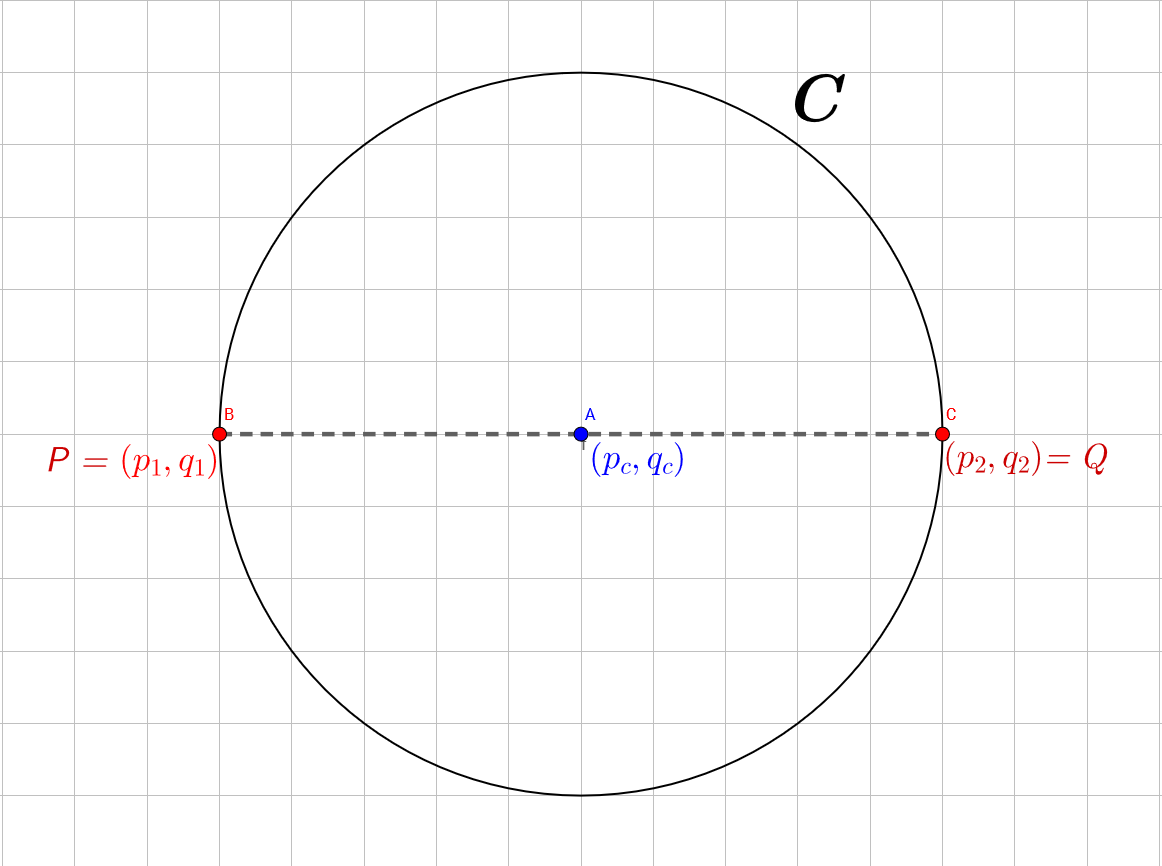
\includegraphics[scale=0.3]{img/p1.png}
            \caption{Ejemplo de Circunferencia \textbf{$C$}.}
            \label{fig:p1}
        \end{figure}
    El segmento punteado es el diámetro horizontal de esta circunferencia, donde el punto $P=(p_1,q_1)$ y $Q=(p_2,q_2)$ son los puntos que definen el diámetro. En este caso el par $(P,Q)$ pertenece al conjunto $E$, notemos que de aqui podemos establecer las propiedades que deben cumplir las coordenadas de $P$ y de $Q$.
    
    En primar lugar, las coordenadas $y$ son iguales (ya que estoy hablando de un diámetro horizontal). Además sin perdida de generalidad podemos decir que la primera coordenada de $P$ debe ser menor que la primera coordenada de $Q$, pues $P$ se ubica a la izquierda de $Q$ en el plano.
    
    Luego el conjunto estudiado se puede escribir por compresión de la siguiente manera
    $$ E=\{(P,Q) ~|~ P=(p_1,q_1),Q=(p_2,q_2), (p_1<p_2) \land (q_1=q_2),~ p_1,q_1,p_2,q_2 \in \Q  \} $$
    De aquí podemos reducir las condiciones que se deben cumplir, obteniendo el siguiente conjunto
    $$ E=\{(P_{(p_1,q_h)},Q_{(p_2,q_h)} ~|~ p_1<p_2,~ p_1,p_2,q_h \in \Q \} $$
    Donde $q_h$ viene a reemplazar el valor de las coordenadas $y$ que tenían el mismo valor para $P$ y $Q$.
    
    Notemos que el radio de estas circunferencias será de la forma $r=\frac{p_2-p_1}{2}$ y el centro será $(\frac{p_1+p_2}{2},q_h)$.
    
    Finalmente, Nos falta demostrar que es infinito numerable.
    
    En efecto, $E$ es infinito pues puedo dejar fijo $p_1=0$, $q_h=0$ y $p_2$ puede recorrer todo $(\Q_{+}\setminus\{ 0\})$, por lo tanto $E$ es infinito, entonces $|E|\geq |\N|$.
    \newpage
    Por otro lado, En el conjunto $E$ estoy guardando una colección de pares ordenados, pues tengo elementos de la forma $(P,Q)$ que realmente es un \emph{objeto} que almacena dos puntos de un plano que viven en $\Q \times \Q$, es decir, $E\subseteq  \Q \times \Q$, entonces $|E|\leq |\Q \times \Q|=|\N|$.
    
    Finalmente por \textbf{Teorema Cantor-Bernstein-Schöeder} se tiene que $|E|=|\N|$, por lo que $E$ es numerable.
    
    Pueden ver otra forma de resolver esto en los siguientes links:
    
    \href{https://drive.google.com/drive/folders/0BxaALcVvHCm5VVlMWGMyRGp0QVU}{\textcolor{BlueViolet}{\underline{Nube Mechona - Malla Vieja - C2 2005}}} y \href{https://www.u-cursos.cl/ingenieria/2016/1/MA1101/5/material_docente/}{\textcolor{BlueViolet}{\underline{P3 - Pauta auxiliar 8 : MA1101-5 - Otoño - 2016}}}
    
    \hyperref[item:P1]{\cfbox{Maroon}{\bf Volver a Enunciado.}}
    %P2
    \item\label{item:S2} Pueden ver la respuesta en \href{https://drive.google.com/drive/folders/0BxaALcVvHCm5VVlMWGMyRGp0QVU}{\textcolor{BlueViolet}{\underline{Nube Mechona - Malla Vieja - C2 2003}}}
    
    \hyperref[item:P2]{\cfbox{Maroon}{\bf Volver a Enunciado.}}
    %P3
    \item\label{item:S3} \textit{Recuerdo: el conjunto imagen se define como $f(A)=\{f(x) : x\in A \}$}
    
    Veamos que $B$ es infinito. Notemos que $A=id_{\R}(A)=f_{1}(A)=\{f_{1}(a): a\in A \}$, por lo que el conjunto $\{f_{1}(a): a\in A \}$ es infinito ya que es igual a $A$. Además es posible notar que $\{f_{1}(a): a\in A \} \subseteq B$, pues basta fijar $n=1$ del conjunto $B$ para obtener este resultado. Por lo tanto $B$ es infinito pues encontramos un subconjunto de $B$ que es infinito. Luego $|B|\geq|\N|$.
    
    Por otro lado, fijando $n$, definamos el conjunto $B_n=\{f_n(a) : a\in A\}=f_n(A)$. Luego podemos construir el conjunto $B$ mediante los $B_n$ de la siguiente forma $$\displaystyle B=\bigcup_{n\in \N}B_n $$
    De aqui si logramos comprobar que $\forall n \in \N, B_n$ es a lo más numerable podemos concluir usando la propiedad de unión numerable de conjuntos a lo más numerables junto con el \textbf{Teorema Cantor-Bernstein-Schöeder}.
    
    En efecto, $B_n$ es a lo más numerable pues podemos definir la función $g:A \to f_n(A)$ tal que $g(x)=f_n(x)$, claramente $g$ es epiyectiva pues estoy definiendo la función $f_n$ desde su dominio hasta su recorrido, por lo que se tiene que $g(A)=cod(g)=f_n(A)$. Luego por propiedad de \textbf{Cardinal de la imagen de un conjunto} tenemos que $|g(A)|\leq|A|$ a esto le sumamos que sabemos que $g(A)=f_n(A)$ y que $A$ es numerable, se cumple que $|f_n(A)|\leq|A|=|\N|$. Como $n$ fue arbitrario se concluye que lo anterior es cierto $\forall n \in \N$, por lo tanto $B_n=f_n(A)$ es a lo más numerable para todo $n$.
    
    Luego $\displaystyle B=\bigcup_{n\in \N}B_n $ es unión numerable de conjuntos a lo más numerables entonces $$\displaystyle |B|=|\bigcup_{n\in \N}B_n |\leq |\N|$$
    Finalmente por el \textbf{Teorema Cantor-Bernstein-Schöeder}, se concluye que $|B|=|\N|$.
    
    Puede ver otras respuesta en \href{https://drive.google.com/drive/folders/0B2BWTqIXpSJsakxLVUNxejQyc1U}{\textcolor{BlueViolet}{\underline{Nube Mechona - C2 2001}}}
    
    \hyperref[item:P3]{\cfbox{Maroon}{\bf Volver a Enunciado.}}
    %P4
    \item\label{item:S4} Entendamos primero el conjunto $A$. Notemos primero que en $A$ viven los elementos de la forma $\frac{p}{q}$ donde $q$ es una potencia de $2$ y $p$ es un natural menor que $q$. Es directo que $p\in N$ y $q\in N$, luego $\frac{p}{q} \in \Q$.

    Ahora bien, en $A$ viven los elementos de la forma $\frac{p}{q} \in \Q$ que cumplen ciertas \textit{\textbf{condiciones}}. Es decir, estoy tomando el conjunto $\Q$ y me estoy quedando con solo algunos elementos. Por lo que $A\subseteq \Q$, esto implica que $|A|\leq |\Q|=|\N|$

    Por otro lado, $A$ es infinito ya que puedo tomar $p=1$ y $q=2^{n}$ puede tomar infinitos valores ya que $n$ recorre todo $\N \setminus \{0,1\}$. Por lo tanto $A$ tiene infinitos elementos, esto implica que $|A|\geq|N|$
    
    Luego por el teorema C-B-S, juntando ambas desigualdades se tiene que $|A|=|\N|$
    
    \hyperref[item:P4]{\cfbox{Maroon}{\bf Volver a Enunciado.}}
    
    %P5
    \item\label{item:S5} Basta notar que como $A\subseteq Z\times Z \longrightarrow |A| \leq |Z\times Z|=|N|$. Luego, falta ver que $A$ es numerable, para eso podemos definir el conjunto $A_{0,n}=\{(0,n) : n\in \N  \}$, claramente este conjunto es infinito ya que $n$ recorre todos los naturales y además $A_{0,n} \subseteq A$. Y como $A_{0,n}$ es infinito entonces $A$ también lo es, entonces $|\N|\leq |A|$. Finalmente por Teorema C-B-S se tiene que $A$ es numerable.
    
    \hyperref[item:P5]{\cfbox{Maroon}{\bf Volver a Enunciado.}}
    
    %P6
    \item\label{item:S6} El conjunto $\mathcal{F}(C,D)$ lo podemos escribir como $D^C$. Recordemos que para conjuntos finitos ocurría lo siguiente:
        \begin{center}
            Para $A$ y $B$ finitos, el conjunto $B^A$ tiene cardinal $|B|^|A|$
        \end{center}
    Por lo que intentaremos hacer lo mismo. Probaremos que $|D^C|=|D^n|$ donde $n$ es el cardinal del conjunto finito $C$, donde $C=\{c_1,\dots,c_n\}$, en otra palabras, probaremos que $|D^C|=|D^{|C|}|$.
    
    Definamos la función $\phi : D^C \to D^n$, donde $n=|C|$, tal que $\phi(f)=(f(c_1),f(c_2),\dots,f(c_n))$, vale decir, $\phi$ toma una función en $D^C$ por lo que $f:C\to D$, y es tal que $\phi(f)$ es una tupla que contiene todas las imágenes que puede generar la función $f$. Falta demostrar que $\phi$ es biyectiva.
    
    \begin{itemize}
        \item \textbf{Inyectiva: } Sea $f,g \in D^C$ tal que 
            \begin{align*}
                \phi(f) &= \phi(g) \\
                (f(c_1),f(c_2),\dots,f(c_n)) &= (g(c_1),g(c_2),\dots,g(c_n))\\
                f(c_i) &=g(c_i) \forall i \in \{1,\dots,n\}
            \end{align*}
            Esto ultimo dice que generan las mismas imágenes con respectivamente las mismas pre-imágenes, esto significa que su conjunto imagen es el mismo. Además, como $f,g \in D^C$, tienen mismo dominio $C$ y mismo codominio $D$. Por lo tanto, como $f$ y $g$ tienen mismo dominio, codominio y conjunto imagen, se concluye que $f=g$ y con esto que $\phi$ es inyectiva.
        \item \textbf{Epiyectiva: } Sea la tupla $(b_1,b_2,\dots,b_n) \in B^n$. Basta con tomar la función $h: C\to D$ tal que $h(c_i)=b_i ~ \forall i \in \{1,\dots,n\}$, de esta forma, $\phi(h)=(h(c_1),h(c_2),\dots,h(c_n))=(b_1,b_2,\dots,b_n)$. Por lo tanto, $\phi$ es epiyectiva.
    \end{itemize}
    
    Como $\phi$ es inyectiva y epiyectiva, se concluye que es biyectiva. Luego como existe biyección entre $D^C$ y $D^n$ con $n=|C|$. Se concluye que $|D^C|=|D^n|$, que es lo mismo que $|D^C|=|D^{|C|}|$. Luego, como $D$ es numerable, se tiene que $D^n$ es numerable, por lo que $D^C$ es numerable.
    
    \hyperref[item:P6]{\cfbox{Maroon}{\bf Volver a Enunciado.}}
    
    %P7
    \item\label{item:S7} Ocupemos el recordatorio. Tomemos un elemento al azar, digamos $x \in B$. Como $\preceq$ es orden total, se tiene que $x\preceq a ~\lor~ a\preceq x$ (puede pasar ambos al mismo tiempo), por lo que equivalentemente $x\in B_1 ~\lor~ x\in B_2$. Esto nos quiere decir que $B= B_1 \cup B_2$. Ahora en adelante probaremos lo que nos piden. Debemos probar que si $B$ es numerable, entonces $B_1$ o $B_2$ es numerable.
    
    Procedamos por contradicción, supongamos que $B_1$ y $B_2$ son finitos. Luego $B=B_1 \cup B_2$ es finito, pero por hipótesis $B$ es infinito numerable $\Rightarrow\!\Leftarrow$. Por lo tanto al menos uno debe ser infinito numerable.
    
    \hyperref[item:P7]{\cfbox{Maroon}{\bf Volver a Enunciado.}}
    
    %P9
    \item\label{item:S8} Puede ver la respuesta en \href{https://drive.google.com/drive/folders/0BxGtZFcrPtd5SnU1Z2JZQTQwOE0}{\textcolor{BlueViolet}{\underline{Nube Mechona - Semestre de primavera - Rapaport 2012-2}}} o bien, en la resolución de los problemas del apunte en la semana 9. 
    
    Esto lo puede encontrar en \href{https://www.u-cursos.cl/ingenieria/2017/1/MA1101/1/material_docente/}{\textcolor{BlueViolet}{\underline{Link a material docente MA1101-1 2018}}} en la sección de material complementario.
    
    \hyperref[item:P8]{\cfbox{Maroon}{\bf Volver a Enunciado.}}
    
    \item\label{item:S9} Notar que $A=\{x\in \R : \exists k\in \Z, \exists i \in \N, x=\dfrac{k}{3^i} \}$. Es decir, los elementos de $A$ son de la forma $\dfrac{k}{3^i}$ donde $k\in \Z$ y claramente $3^i \in \N$, es decir, $x\in \Q$. Por lo tanto $A\subseteq \Q$ y con esto $|A|\leq |\Q|=|\N|$.
    
    Por otro lado, claramente $A$ es infinito ya que podemos fijar $i=0$ con lo que obtenemos los elementos de la forma $x=\dfrac{k}{3^0}=k$ y $k$ puede recorrer todo $\Z$ por lo tanto $A$ es infinito, es decir, $|N|\leq |A|$.
    
    Finalmente por teorema C-B-S se concluye que $|A|=|\N|$.
    
    \hyperref[item:P9]{\cfbox{Maroon}{\bf Volver a Enunciado.}}
    
    %P10
    \item\label{item:S10} Puede ver la respuesta en \href{https://drive.google.com/drive/folders/0BxGtZFcrPtd5SnU1Z2JZQTQwOE0}{\textcolor{BlueViolet}{\underline{Nube Mechona - Semestre primavera - Varas 2010-2}}}
    
    \hyperref[item:P10]{\cfbox{Maroon}{\bf Volver a Enunciado.}}
    
    %P11
    \item\label{item:S11} Pueden ver la respuesta en \href{https://drive.google.com/drive/folders/0BxaALcVvHCm5VVlMWGMyRGp0QVU}{\textcolor{BlueViolet}{\underline{Nube Mechona - Malla Vieja - C2 2000}}} o bien, en la resolución de los problemas del apunte en la semana 9. 
    
    Esto lo puede encontrar en \href{https://www.u-cursos.cl/ingenieria/2017/1/MA1101/1/material_docente/}{\textcolor{BlueViolet}{\underline{Link a material docente MA1101-1 2018}}} en la sección de material complementario.
    
    \hyperref[item:P11]{\cfbox{Maroon}{\bf Volver a Enunciado.}}
    
    %P12
    \item\label{item:S12} Semana 9 de la resolución de los problemas del apunte. 
    
    Esto lo puede encontrar en \href{https://www.u-cursos.cl/ingenieria/2017/1/MA1101/1/material_docente/}{\textcolor{BlueViolet}{\underline{Link a material docente MA1101-1 2018}}} en la sección de material complementario.
    
    \hyperref[item:P12]{\cfbox{Maroon}{\bf Volver a Enunciado.}}
    
    %P13
    \item\label{item:S13} Semana 10 de la resolución de los problemas del apunte. 
    
    Esto lo puede encontrar en \href{https://www.u-cursos.cl/ingenieria/2017/1/MA1101/1/material_docente/}{\textcolor{BlueViolet}{\underline{Link a material docente MA1101-1 2018}}} en la sección de material complementario.
    
    \hyperref[item:P13]{\cfbox{Maroon}{\bf Volver a Enunciado.}}
    %P14
    
    \item\label{item:S14} Notemos primero que debemos demostrar que una \textbf{unión} entre dos conjuntos es numerable, donde ya sabemos por enunciado que uno de ellos es numerable. Es decir, debemos probar que $X \cup -X$ es numerable y sabemos que $X$ es numerable. Si logramos demostrar que $-X$ es numerable, podríamos ocupar que \textbf{unión de numerables es numerable}. Así que abordemos el problema por acá.
    
    Demostremos que $-X$ es numerable.
    En efecto, definamos la función $f: X \to -X$ tal que $f(x)=-x$. Esta función es claramente una biyección ya que es una recta con pendiente $-1$ y coeficiente de posición igual a $0$ y de introducción al cálculo sabemos que una recta es biyectiva (Compruébelo, aunque no es necesario).
    
    Luego, encontré una función biyectiva entre $X$ y $-X$ entonces $|X|=|-X|$ pero $|X|=|\N|$, por lo tanto $|-X|=|\N|$, es decir $-X$ es numerable al igual que $X$.
    
    Ahora como $X$ y $-X$ son numerables, la unión de ellos también lo será, por lo que se concluye que $|X\cup -X|=|\N|$
    
    \hyperref[item:P14]{\cfbox{Maroon}{\bf Volver a Enunciado.}}
    
    %P15
    \item\label{item:S15} Notemos que en $A=\{ r+s\sqrt{2}: r,s \in \Q \}$, la variable $r$ y la variable $s$ recorren todo $\Q$. Así que aprovechemos esto y tratemos de escribir el conjunto $A$ como una \textbf{unión numerable de conjuntos numerables}.
    
    Procedamos de la siguiente forma (esto se puede hacer siempre):
    
    Fijemos la variable $s$ en un valor $\overline{s} \in \Q$, luego podemos definir el conjunto $$ A_{\overline{s}}=\{ r+\overline{s}\sqrt{2}: r \in \Q \}$$
    Donde aquí hemos tomado la definición de $A$ y hemos fijado $s$ en $\overline{s}$.
    
    Luego, tenemos que responder a la siguiente pregunta. \textbf{¿Como puedo recuperar la definición del conjunto $A$ en términos de mi nuevo conjunto $A_{\overline{s}}$?}.
    Bueno, me basta con realizar lo siguiente
    $$\displaystyle  A=\bigcup_{\overline{s}\in \Q } \{ r+\overline{s}\sqrt{2}: r \in \Q \}= \bigcup_{\overline{s}\in \Q} A_{\overline{s}} $$
    Ya que con la unión garantizo que $\overline{s}$ recorra todo $\Q$ (notar que ahora la barrita sobre $s$ da lo mismo pues vamos a tomar diferentes valores de $s$).
    
    Luego, como $\displaystyle A=\bigcup_{s\in \Q} A_{s}$, se tiene que $A$ es una unión numerable de conjuntos los cuales no sabemos si son numerables. Primero, es una unión numerable pues el índice recorre un conjunto numerable que es $\Q$, ahora veamos que $A_s$ es numerable para todo $s$.
    
    En efecto, consideremos la función $g: \Q \to A_s$ tal que $g(r)=r+\sqrt{2}s$.
    Por simple construcción esta función es biyectiva, ya que es una recta de pendiente $1$ y coeficiente de posición $r\sqrt{2}$. Luego $g$ es biyectiva y con esto $|\Q|=|A_s|$, pero como $|\Q|=|\N|$ entonces $|A_s|=|\N|$, es decir $A_s$ es numerable, donde el $s$ que ocupamos fue arbitrario (nunca dijimos nada sobre $s$) por lo que este resultado se obtiene para todo $s \in \Q$.
    
    Por lo tanto, tenemos que $A$ es una unión numerable de conjuntos numerables ya que,  $\displaystyle A=\bigcup_{s\in \Q}A_s$. Por lo tanto $A$ es numerable.
    
    \hyperref[item:P15]{\cfbox{Maroon}{\bf Volver a Enunciado.}}
    
    %P16
    \item\label{item:S16} Siguiendo la indicación, basta notar que $H_b=\{(a,b) :a\in A\}$ con $b\in B$ fijo. Es decir $H_b=A\times \{b\}$. De esta manera $A\times B= \bigcup_{b\in B} H_b$, vale decir, unimos todos los conjuntos de la forma $H_b$ fijando distintos $b$.
    
    Luego $A\times B$ es igual a la unión numerable de conjuntos de la forma $H_b$, si logramos demostar que $H_b$ es numerable podremos concluir.
    
    En efecto, sea $b \in B$ fijo, debemos probar que $H_b$ es numerable, lo compararemos con $A$. Definimos la función $f: A\to H_b$ tal que $f(a)=(a,b)$. Se deja propuesto ver que $f$ es biyectiva. Luego, como $f$ es biyección, $|A|=|H_b|$ y como $A$ es numerable, $H_b$ también lo es.
    
    Por lo tanto, como $A\times B = \bigcup_{b\in B} H_b$, se tiene que $A\times B$ es unión numerable de conjuntos numerables por lo tanto $A\times B$ es numerable.    
    
    \hyperref[item:P16]{\cfbox{Maroon}{\bf Volver a Enunciado.}}
    
    %P17
    \item\label{item:S17} Motivados por la pregunta anterior, podemos fijar $b\in \Q$ y definir el conjunto $H_b=\{a^b : a\in \N \setminus \{0\}\}$. De esta forma $H= \bigcup_{b\in \Q}H_b$.
    
    Estamos en la misma posición que antes, tenemos una unión numerable de conjuntos que no sabemos que cardinal tienen. Debemos ser capaces de probar que para todo $b$ se tiene que $|H_b|\leq |N|$ para que nuestro problema siga teniendo sentido (pues de lo contrario, existe un $H_{b'}$ no numerable por lo que $H$ seria no numerable). Para esto, definamos la función $f: \N\setminus \{0\} \to H_b$ tal que $f(n)=n^b$ donde $b \in \Q$ es el racional fijo. Claramente esta función es epiyectiva ya que si escogemos un $y\in H_b$ cualquiera, por definición debe existir al menos un natural $a\neq 0$ tal que $a^b=y$. Luego basta tomar $n=a$ para que $f(n)=n^b=a^b=y$. Es decir, $f$ es epiyectiva y con esto $|H_b|\leq |\N|$.
    
    En virtud de lo anterior $H = \bigcup_{b\in \Q}H_b$ es una unión numerable de conjuntos a lo más numerables, por lo que $|H|\leq |\N|$. Para concluir falta ver que al menos un conjunto que participa en la unión es infinito numerable. En efecto, si $b=1$, se tiene que $H_1=\{ a : a\in \N \setminus \{ 0 \}$, es decir $|H_1|=|\N \setminus \{0\}|=|\N|$. Por lo que existe un conjunto que participa en la unión que es infinito numerable. Luego, como $H_1 \subseteq H$ entonces $|\N|=|H_1|\leq |H|$. Finalmente por teorema C-B-S se concluye que $|H|=|\N|$.
    
    \hyperref[item:P17]{\cfbox{Maroon}{\bf Volver a Enunciado.}}
    
    %P18
    \item\label{item:S18} Pueden ver la respuesta en \href{https://drive.google.com/drive/folders/0B2BWTqIXpSJsQ01SdE9YVDlOZzA}{\textcolor{BlueViolet}{\underline{Nube Mechona - C4 2009}}}
    
    \hyperref[item:P18]{\cfbox{Maroon}{\bf Volver a Enunciado.}}
    
    %P19
    \item\label{item:S19} Pueden ver la respuesta en \href{https://drive.google.com/drive/folders/0B2BWTqIXpSJsQ01SdE9YVDlOZzA}{\textcolor{BlueViolet}{\underline{Nube Mechona - C4 2010}}}
    
    \hyperref[item:P19]{\cfbox{Maroon}{\bf Volver a Enunciado.}}
    
    %P20
    \item\label{item:S20} Pueden ver la respuesta en \href{https://drive.google.com/drive/folders/0B2BWTqIXpSJsQ01SdE9YVDlOZzA}{\textcolor{BlueViolet}{\underline{Nube Mechona - C4 2013}}}
    
    \hyperref[item:P20]{\cfbox{Maroon}{\bf Volver a Enunciado.}}
    
    \item\label{item:S21} Entendamos el conjunto $\mathcal{F}$.\\
        Los elementos de $\mathcal{F}$ son las funciones de $f:\N \to  \N$ tal que 
        $$f(0)=0 ~~~~\land~~~~ f(n+1)=f(n)+d  $$
        Esto es una recursión, así que tratemos de hacer desaparecer la recursión y llegar a una formula explicita de la función $f$ para poder interpretar el problema más claramente. Así que veamos cuanto vale $f(1), f(2),\dots,f(n)$.
            \begin{align*}
                f(1)&=f(0)+d =0+d =d\\
                f(2)&=f(1)+d =d+d =2d\\
                f(3)&=f(2)+d =2d+d =3d
            \end{align*}
        Así que de esta forma, podemos conjeturar que $\forall n\in \N,~f(n)=nd$. Demostrémoslo por inducción
        
        \textbf{\underline{Caso Base}:} $n=0$. En efecto, $f(0)=0\cdot d=0$ y por definición del conjunto $\mathcal{F}$, $f(0)=0$. Por lo que se cumple el caso base.
        
        \textbf{\underline{Hipótesis inductiva}:} supongamos que $\exists k\in \N, f(k)=kd$ es verdadero.
         
        \textbf{\underline{Paso inductivo}:} debemos probar que $f(k+1)=(k+1)d$.
        En efecto, notemos que por la definición recursiva $f(k+1)=f(k)+d$ y por \textbf{Hipótesis inductiva} se tiene que $f(k)=kd$. Entonces 
            $$ f(k+1)=f(k)+d=kd +d=(k+1)d $$
        Por lo tanto, la inducción fue un éxito y se concluye que $\forall n\in \N,~f(n)=nd$
        
        Ahora reescribamos el conjunto que estamos estudiando.
        
        $$\Longrightarrow \mathcal{F}=\{f:\N\to \N ~|~ \exists d\in \N, \forall n\in \N f(n)=nd \}$$
        
        Es decir el conjunto $\mathcal{F}$ es el conjunto de las funciones, las cuales son rectas, de $\N$ en $\N$ tal que su pendiente es $d\in \N$ y su coeficiente de posición es $0$. Ahora si estamos en condiciones de probar que el conjunto es numerable.
        
        En efecto, definamos la función $\varphi: \mathcal{F} \to \N$ tal que $\varphi(f_d)=d$, es decir mi función $\varphi$ toma una recta de pendiente $d$ y al evaluarlo da como resultado su pendiente. Demostremos que $\varphi$ es biyectiva.
        
        \textbf{\underline{Inyectividad: }}Sea $f_{d},g_{d'} \in \mathcal{F}$ tal que $\varphi(f_{d})=\varphi(g_{d'})$. Entonces
        
         \begin{alignat}{2}
                &\Longrightarrow\quad &\varphi(f_d)  &= \varphi(g_{d'})\notag\\ 
                &\Longrightarrow  & d &= d' \notag\\  
                &\Longrightarrow & n\cdot d &= n\cdot d' \notag\\
                &\Longrightarrow & f_d &= g_{d'} \notag
            \end{alignat}
        
        Por lo tanto es inyectiva.
        
        \textbf{\underline{Epiyectividad: }} Si quiero obtener $d\in \N$, me basta tomar la función $f:\N \to \N$ tal que $f_{d}(n)=dn$, ya que $\varphi(f_d)=d$.
        Por lo tanto es epiyectiva.
        
        Luego $\varphi$ es biyectiva entre $\mathcal{F}$ y $\N$, por lo tanto $|\mathcal{F}|=|\N|$, es decir $\mathcal{F}$ es numerable.
        
        \hyperref[item:P21]{\cfbox{Maroon}{\bf Volver a Enunciado.}}

    %P22    
    \item\label{item:S22} Pueden ver la respuesta en \href{https://drive.google.com/drive/folders/0B2BWTqIXpSJsQ01SdE9YVDlOZzA}{\textcolor{BlueViolet}{\underline{Nube Mechona - C4 2016}}}
    
    \hyperref[item:P22]{\cfbox{Maroon}{\bf Volver a Enunciado.}}
    
    %P23
    \item\label{item:S23} Como $|A|<|B$ entonces existe inyección $f$ de $A$ en $B$ pero no biyección. y como $B\subseteq C$ entonces $|B|\leq |C|$ es decir, existe inyección $g$ de $B$ en $C$. Claramente, por composición de funciones inyectivas, $g \circ f : A\to C$ es inyección, entonces $|A|\leq |C|$. Falta ver que no hay biyección entre $A$ y $C$. Supongamos por contradicción que hay biyección $h:C\to A$. Como $g: B\to C$ es inyectiva (la que ocupamos anteriormente en la composición), se tiene que $h\circ g: B\to A$ es inyección pues es composición de funciones inyectivas. Luego, $|B|\leq |A|$ y por hipótesis $|A|<|B|$ lo que es una contradicción ya que de ser asi se tendria que $|A|=|B|. ~ \Rightarrow\!\Leftarrow$
    
    
    \hyperref[item:P23]{\cfbox{Maroon}{\bf Volver a Enunciado.}}
    
    %P24
    \item\label{item:S24} En desarrollo
    
    \hyperref[item:P24]{\cfbox{Maroon}{\bf Volver a Enunciado.}}
    
    %P25
    \item\label{item:S25} \begin{enumerate}
\item Definamos la función $f: E_m \to (\Z\setminus \{0\} )\times \Z^{m}$ como:
$$
f(a_mx^m+a_{m-1}x^{m-1}+\dots+a_1x+a_0 )=(a_m,a_{m-1},\dotso, a_1,a_0))
$$
Esta función es biyectiva. Con esto concluimos que $|E_m|=|(\Z\setminus \{0\} )\times \Z^{m}|=|\N| $.
\item Sea $E$ el conjunto de las ecuaciones algebraicas. Notemos que $E = \bigcup\limits_{n\in \N}E_n$ luego $E$ es una unión numerable de conjuntos numerables y por tanto $E$ es numerable.

\item Definamos $\mathcal{A} $ como el conjunto de números algebraicos, separemos la demostración en dos partes:
\begin{itemize}
\item $(|\mathcal{A}|\leq |\N|)$:
Notemos que:
$$
\mathcal{A}=\bigcup_{e(x) \in E }  \{  x\in \R : e(x)=0  \}
$$
Luego $\mathcal{A}$ es una unión numerable de a lo más numerables, por tanto $\mathcal{A}$ es a lo más numerable, es decir $|\mathcal{A}|\leq |\N|$.
\item $(|\N|\leq |\mathcal{A}|)$:\\
Notemos que como:
$$
x-m=0
$$
Es una ecuación algebraica para $m\in \N$, tenemos que $\N \subseteq \mathcal{A}$ y por tanto:
$$
|\N|\leq |\mathcal{A}|
$$
\end{itemize}
Por el Teorema de Cantor-Bernstein-Schröder concluimos que $|\mathcal{A}|=|\N|$.
\item Llamemos $\mathcal{T}$ al conjunto de los números trascendentes, notemos que $\mathcal{T}=\mathcal{A}^c$. 
Demostremos que $\mathcal{T}$ tiene que ser un conjunto infinito no numerable, pues si fuera a lo más numerable tenemos que:
$$
|\R |= |\mathcal{A}\cup \mathcal{T}|\leq |\N|
$$
Lo que contradice el hecho que $|\N|<|\R|$. Por tanto $|\N|<|\mathcal{T}|$.
\item Como $|\N|<|\mathcal{T}|$, $\mathcal{T}$ no puede ser vacío.
\end{enumerate}
    
    
    \hyperref[item:P25]{\cfbox{Maroon}{\bf Volver a Enunciado.}}
\end{enumerate}




































\end{document}